\documentclass{standalone}

\usepackage{tikz}
\usepackage{pgfplots,tikz-3dplot}
\makeatother
\begin{document}
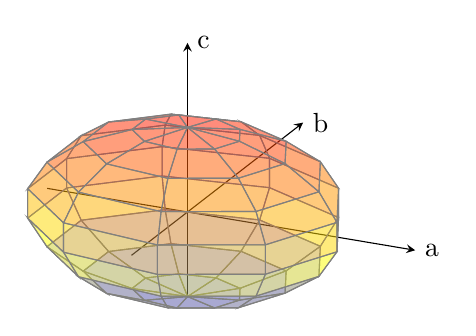
\begin{tikzpicture}
    \begin{axis}[%
        % width=0.8\textwidth,
        % axis equal,
        axis lines = center,
        x label style={at={(axis cs:3,0,0)},anchor=west},
        y label style={at={(axis cs:0,4,0)},anchor=west},
        z label style={at={(axis cs:0,0,1)},anchor=west},
        xlabel = {a},
        ylabel = {b},
        zlabel = {c},
        xmax=3,
        ymax=4,
        zmax=1,
        ticks=none,
        % colormap={}{ gray(0cm)=(0.8); gray(1cm)=(0);}
    ]
    \addplot3[%
        fill opacity=0.3,
        surf,
        % shader=flat,
        faceted color=gray,
        % shader=interp,
        %shader=faceted,
        %shader=flat corner,
        % shader=flat mean,
        % shader=faceted interp,
        samples = 10,
        domain=0:2*pi,y domain=0:pi,
        z buffer=sort
        ]
        ({2*cos(deg(x))*sin(deg(y))}, {2*sin(deg(x))*sin(deg(y))}, {0.5*cos(deg(y))});
    \end{axis}
%
\end{tikzpicture}
\end{document}
